Nous pr\'esentons les r\'esultats obtenus avec la distance de Pearson.
\newline
Les grandeurs physiques collect\'ees proviennent du {\em data center Champlan} sont au nombre de $10$. Elles sont regroup\'ees dans les syst\`emes triphas\'e et monophas\'e.
Dans les s\'eries de mesures  provenant des arcs en triphas\'e, nous remarquons qu'il y a toujours des mesures sur une phase et les autres phases ne contiennent aucune mesure. Il n'y a aucune mesure sur deux phases simultan\'ement et lorsqu'il  existe des mesures, les $i$ premi\`eres mesures sont sur la phase $1$, les $n-i$ mesures sont sur la phase $2$. 
Les autres grandeurs ne contiennent des mesures 
soit dans les $i$ premiers instants de temps, 
soit dans les $n-i$ derniers instants de temps. 
Il est alors difficile d'exploiter ces mesures partielles.
% parler du seule tgbt qui est en monophas\'e
Quant au syst\`eme monophas\'e, $20\%$ des mesures des puissances r\'eactives $Q$ et apparentes $S$ dans une s\'erie temporelle sont manquantes, $25\%$ des mesures ne correspondent pas aux formules de calculs th\'eoriques. 
Le nombre de valeurs \`a consid\'erer dans les s\'eries des grandeurs n'est pas assez significative pour calculer les similarit\'es parce que la distance de Pearson est sensible \`a la dimension de la s\'erie \`a cause de sa relation avec le coefficient de Pearson. Il est difficile de trouver de possibles comportements identiques \`a partir des hypoth\`eses de corr\'elation avec des s\'eries de grandes tailles et autant de valeurs absentes.
\newline
% 2- description du reseau de champlan et presentation du reseau (affichage) 
Nous consid\'erons un sous-r\'eseau \'electrique de {\em Champlan} dans lequel 
\begin{itemize}
	\item La grandeur s\'electionn\'ee poss\`ede des valeurs quelque soit le syst\`eme (triphas\'e ou monophas\'e). La grandeur qui respecte cette r\`egle est la {\em puissance $P$}.
	\item Les s\'eries temporelles correspondent \`a un mois de mesures. 
		Dans chaque s\'erie, nous avons en moyenne $15\%$ de valeurs manquantes que nous remplacons par la valeur moyenne de chaque s\'erie.
	\item L'application de la loi des noeuds est possible.
	\item Aucun \'equipement n'est aliment\'e par un onduleur. La pr\'esence d'un onduleur modifie le profil de consommation d'un arc car l'onduleur recr\'ee le signal en attribuant des puissances diff\'erentes. Cela implique que nous n'avons pas des m\^emes variations.
	 
\end{itemize}
Un exemple de ce sous-r\'eseau est illustr\'e dans la figure \ref{sousReseauChamplan} dans lequel nous avons $31$ \'equipements. Les sources sont identifi\'ees par {\em TGBT} (TGBT1, TGBT2, TGBT4) et $GF$(1,2) d\'esigne le groupe froid qui g\`ere la climatisation. Les tableaux sont {\em DD205, DD206, DD105, DD106, DD108, MSC3, R486, R481, CVC1 et CVC2}. Les baies sont {\em R491, R488, R484A, R484B, R042, R483, R487, R492, R490, R493, R494}. Les onduleurs sont indiqu\'es par {\em OND} (1,2,RG). Les \'equipements {\em TGBT} sont aliment\'es par une source externe au data center, le fournisseur d'\'electricit\'e r\'egional {\em Enedis}.  
% ---- figure sous-reseau champlan
\begin{figure}[htb!] 
\centering
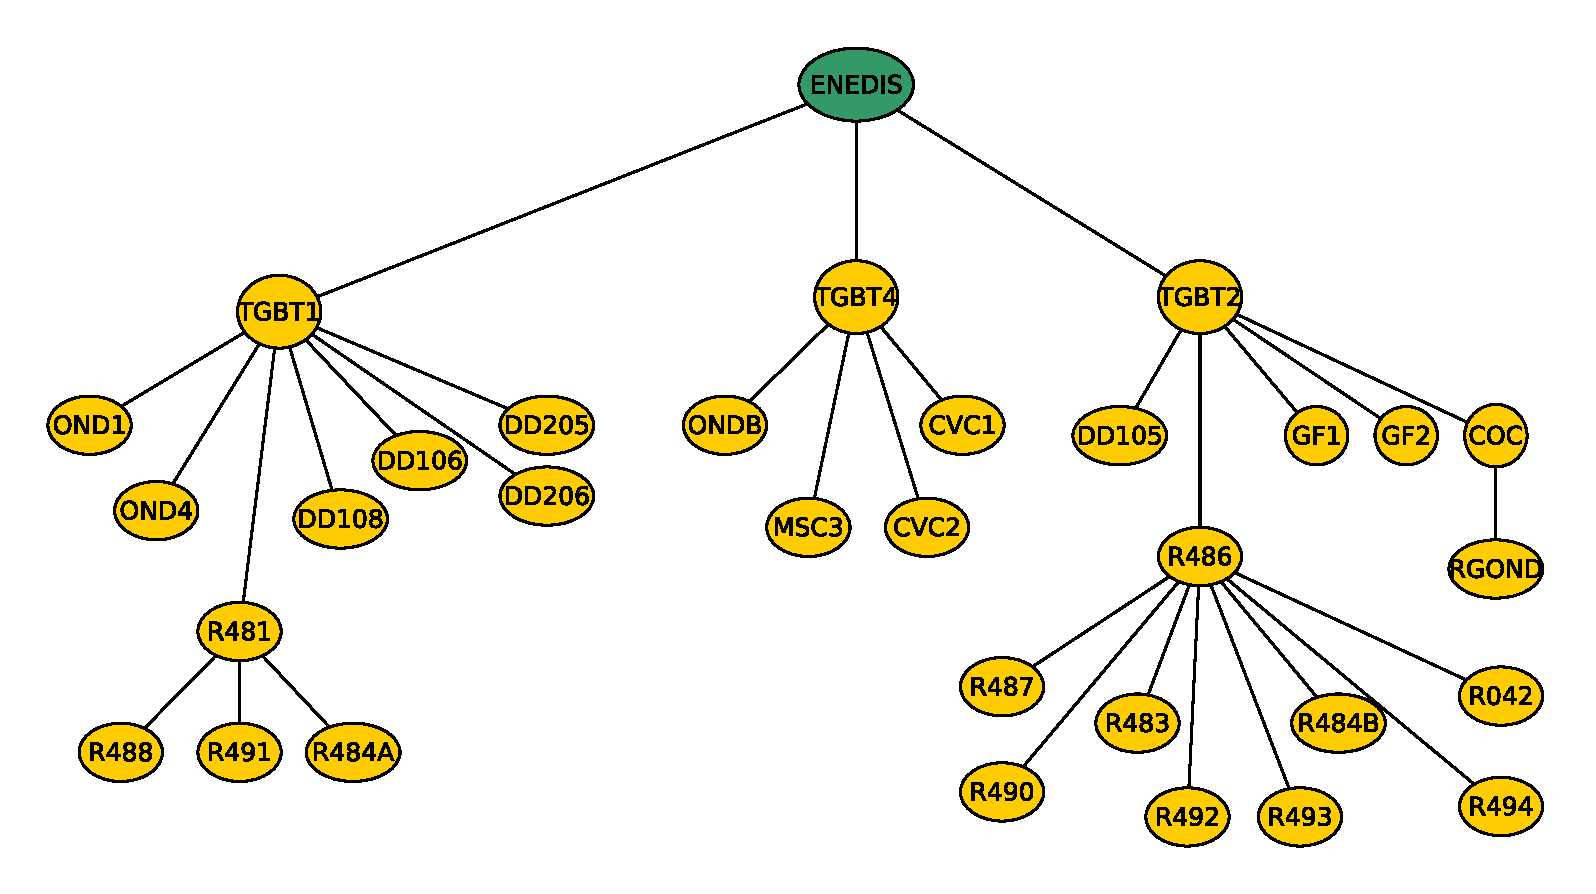
\includegraphics[scale = 0.65]{sousReseauChamplan.eps}
\caption{Le sous-r\'eseau de Champlan \'etudi\'e : Les sources sont {\em TGBT1, TGBT2, TGBT4}. $GF$(1,2) d\'esigne le groupe froid qui g\`ere la climatisation. 
Les tableaux sont {\em DD205, DD206, DD105, DD106, DD108, MSC3, R486, R481, CVC1 et CVC2}. 
Les baies sont {\em R491, R488, R484A, R484B, R042, R483, R487, R492, R490, R493, R494}. Les onduleurs sont indiqu\'es par {\em OND1,OND2,RGOND}. 
Les \'equipements {\em TGBT} sont aliment\'es par une source externe au data center, le fournisseur d'\'electricit\'e r\'egional {\em Enedis}.
}
\label{sousReseauChamplan}
\end{figure}
% ---- figure sous-reseau champlan.
\newline

% 3-  coefficients de similarite 
Nous allons calculer la corr\'elation entre les arcs du {\em sous-r\'eseau de Champlan} en supposant que {\em deux arcs incidents \`a un \'equipement sont fortement corr\'el\'es et deux arcs non corr\'el\'es ne poss\`edent aucun \'equipement en commun}.
Chaque arc est identifi\'e par deux \'equipements, celui qui fournit l'\'electricit\'e ($x$) et celui qui en consomme ($y$). Nous d\'esignons par convention $x->y$, l'arc entre $x$ et $y$. Par exemple, l'arc entre $TGBT1$ et $R481$ est not\'e $TGBT1->R481$. 
\newline
Soient trois arcs $x->y$ et $y->z$ et $t->u$. 
Le coefficient de similarit\'e $corr(x->y,y->z) = 1$ signifie que les arcs $x->y$ et $y->z$  ont les m\^emes profils de consommation, partagent le sommet $y$ et sont fortement corr\'el\'es. De m\^eme, le coefficient $corr(x->y,t->u) = 0$ indique que les arcs  $x->y$ et $t->u$ ne sont pas corr\'el\'es c'est-\`a-dire qu'ils n'ont pas de sommet en commun et que leurs profils de consommation sont diff\'erents.
\newline

% ---- figure sous-reseau champlan
\begin{figure}[htb!] 
\centering
\includegraphics[scale = 0.55]{distribution_0_1_distance_pearson.jpeg}
\caption{Distribution des coefficients des similarit\'es selon les arcs qui sont incidents.
$cases\_1$ d\'esigne les arcs incidents et $cases\_0$ d\'esigne les arcs non incidents dans le {\em sous-r\'eseau de Champlan}.
Le coefficient de similarit\'e $0.1$ indique toutes les valeurs dans l'intervalle $[0.1, 0.2[$.
}
\label{distribution_0_1_distance_pearson}
\end{figure}
% ---- figure sous-reseau champlan.
% 4 erreur de similarite et categorisation de ces erreurs 
Nous disposons de la topologie \'electrique r\'eelle de {\em Champlan}.
Nous comparons  les coefficients de similarit\'e  calcul\'es par rapport aux arcs qui sont incidents dans la topologie de {\em Champlan}.
Pour ce faire, nous pr\'esentons, dans la figure \ref{distribution_0_1_distance_pearson}, les distributions des arcs incidents et non incidents  en fonction des coefficients de similarit\'e. Les arcs non incidents sont d\'esign\'es par $cases\_0$ et les arcs incidents par $cases\_1$.
	% arcs non adjacents : prkoi on a des coeff = 1?
		% ---- figure  profils_consommation_cases_0_similarite_1
		\begin{figure}[htb!] 
		\centering
		\includegraphics[scale = 0.65]{profils_consommation_cases_0_similarite_1.jpeg}
		\caption{ Profils de consommation des paires d'arcs n'ayant aucun \'equipement en commun. 
		En haut \`a gauche, nous avons les courbes des arcs $TGBT2->GF2$, $TGBT1->DD106$. 
		En haut \`a droite, les courbes des arcs $TGBT2->GF2$, $TGBT1->DD108$. 
		En bas \`a gauche, les courbes des arcs $R486->R487$, $R481->R488$.
		En bas \`a droite,  les courbes des arcs  $TGBT1->DD205$, $TGBT4->MSC3$
		}
		\label{profils_consommation_cases_0_similarite_1}
		\end{figure}
%		\FloatBarrier
		% ---- figure  profils_consommation_cases_0_similarite_1
	La distribution des arcs non incidents est asym\'etrique vers la gauche. Cela est normal puisque nous avons suppos\'e que les arcs non incidents ont des coefficients de similarit\'e qui sont proche de $0$. 
	Cependant, nous avons quatre paires d'arcs qui ont des coefficients $corr(x->y,y->z) = 1$. La figure \ref{profils_consommation_cases_0_similarite_1} pr\'esente les profils de consommation de ces quatre paires d'arcs. Nous constatons que :
	\begin{itemize}
		\item Les arcs $R486->R487$ et $R481->R488$ ont des profils oppos\'es et en appliquant la valeur absolue sur les valeurs de chaque s\'erie, les profils se superposent. Il n'y a aucune corr\'elation entre cette paire d'arcs. 
		\item Les arcs $TGBT1->DD205$ et $TGBT4->MSC3$ ont leurs profils qui se superposent et la corr\'elation de Pearson entre ces s\'eries est alors nulle.
		\item Les paires d'arcs $TGBT2->GF2$ et $TGBT1->DD106$ ont des courbes qui ont plusieurs points d'intersection. \`A ces points, le coefficient de similarit\'e est nul et est proche de $0$ au voisinage de ces points. La corr\'elation de Pearson entre ces s\'eries est alors nulle. 
	\end{itemize}
	Cela implique que le coefficient de similarit\'e est \'egal \`a $corr(x->y,y->z) = 1$ entre ces paires d'arcs $x->y,y->z$ par l'\'equation \ref{personDistance} alors que ces arcs n'ont aucun sommet en commun dans le graphe de la figure \ref{sousReseauChamplan}.
	Ces erreurs de corr\'elation sont introduites par la m\'ethode de calcul des coefficients.
	\newline  
	% arcs adjacents : prkoi on a des coeff = 0.1?
		% ---- figure profils_consommation_cases_1_similarite_0.1
		\begin{figure}[htb!] 
		\centering
		\includegraphics[scale = 0.65]{profils_consommation_cases_1_similarite_01.jpeg}
		\caption{ Profils de consommation des paires d'arcs ayant un \'equipement en commun. 
		les arcs $TGBT2->GF2$ et $TGBT2->COC$ partagent l'\'equipement $TGBT2$.}
		\label{profils_consommation_cases_1_similarite_01}
		\end{figure}
		% ---- figure  profils_consommation_cases_1_similarite_0.1
	En ce qui concerne la distribution des coefficients de similarit\'e des arcs incidents ($cases\_1$), elle est aussi asym\'etrique \`a gauche avec un pic  pour les coefficients appartenant \`a l'intervalle $[0.1,0.2[$. Pour comprendre cette distribution, nous repr\'esentons les profils de consommation de certaines paires d'arcs incidents  ayant leur coefficient de similarit\'e appartenant \`a  l'intervalle $[0.1,0.2[$ dans la figure \ref{profils_consommation_cases_1_similarite_01}.  
	Dans ces repr\'esentations, il y a toujours une courbe constante et sa pr\'esence est due \`a l'impossibilit\'e de collecter des donn\'ees \`a cause d'une panne. 
	Cette s\'erie contient alors des valeurs nulles. Il y'a aussi la fourniture d'\'energie dans les branches. En effet, la source ne fournit que la quantit\'e d'\'energie demand\'ee par un \'equipement. Les s\'eries des arcs sont diff\'erentes et la distance de Pearson est la plus faible ($corr(x->y,y->z) = 0.1$). 
	Dans ce cas, les erreurs sont introduites par les donn\'ees et le fonctionnement du r\'eseau.
\newline	
Dans les cas d'erreurs de similarit\'e \'enonc\'ees plus haut, nous ne pouvons pas les \'eviter  pendant le calcul des coefficients parce que le m\'ecanisme de r\'ecup\'eration des donn\'ees est d\'efaillant et  l'arr\^et de la consommation d'\'electricit\'e d'une branche est masqu\'e par la mise en service de plusieurs serveurs dans une baie appartenant \`a une autre branche.
\newline 

% matrice de correlation et type d erreurs
Les coefficients de similarit\'e sont regroup\'es dans une matrice sym\'etrique  carr\'ee de dimension $N \times N$ avec $N$ le nombre d'arcs dans le {\em sous-r\'eseau de Champlan}.
Les lignes et les colonnes de la matrice sont les arcs du sous-r\'eseau. Chaque case de la matrice contient un coefficient de similarit\'e entre deux arcs. Les cases de la diagonale de la matrice contiennent les coefficients d'un arc avec lui-m\^eme et sont \'egales \`a $0$.  
Cette matrice est appel\'ee {\em matrice de corr\'elation} et se note $M_c$.
Sur cette matrice, diff\'erentes valeurs de seuils $s \in [0,1]$ sont test\'ees dans le but de d\'eterminer la matrice d'adjacence $M_{c,s}$ du {\em sous-r\'eseau de Champlan}. 
Des arcs $x->y$ et $x->z$ dont leur coefficient $corr(x->y, x->z) \ge s$ ont leur case $M_{c,s}[x->y, x->z] = 1$ sinon $M_{c,s}[x->y, x->z] = 0$ si $corr(x->y, x->z) < s$. 
La figure \ref{distrib_relationAdjacence_seuils_distancePerson} pr\'esente les distributions des relations d'incidences entre les arcs apr\`es l'application  des seuils sur la matrice de corr\'elation. Pour un seuil donn\'e, les relations d'incidences sont regroup\'ees en $4$ cat\'egories :
\begin{itemize}
	\item Les incidences {\em vraies positives} : il existe un sommet en commun entre les arcs et la case associ\'ee de la paire d'arcs $[x->y, x->z]$ est $M_{c,s}(x->y, x->z) = 1$. 
	\item Les incidences {\em vraies n\'egatives} : il n'existe aucun sommet en commun entre les arcs et la case associ\'ee de la paire d'arcs $[x->y, x->z]$ est $M_{c,s}(x->y, x->z) = 0$. 
	\item Les incidences {\em fausses positives} :  il n'existe aucun sommet en commun entre les arcs et la case associ\'ee de la paire d'arcs $[x->y, x->z]$ est $M_{c,s}(x->y, x->z) = 1$. 
	\item Les incidences {\em fausses n\'egatives} :  il existe un sommet en commun entre les arcs et la case associ\'ee de la paire d'arcs $[x->y, x->z]$ est $M_{c,s}(x->y, x->z) = 0$. 
\end{itemize}
Les incidences {\em fausses positives} et {\em fausses n\'egatives} constituent des {\em erreurs d'incidences} dans la matrice d'adjacence $M_{c,s}$. Nous consid\'erons aussi certaines incidences {\em vraies positives}  et {\em vraies n\'egatives} comme les {\em erreurs d'incidences}.
Chaque graphique affiche les erreurs d'incidences associ\'ees \`a un seuil. Par exemple, dans le graphique {\em VraiPositive\_ErreurAdjacence} de la figure \ref{distrib_relationAdjacence_seuils_distancePerson} nous avons $17$ paires d'arcs partageant un sommet pour un seuil $s=0.4$. De m\^eme, nous avons $57$ paires d'arcs n'ayant aucun sommet en commun pour un seuil $s=0.4$ dans le graphique {\em fauxNegatives\_ErreurAdjacence} de la figure \ref{distrib_relationAdjacence_seuils_distancePerson}. 
Nous observons qu'il n'existe aucun seuil qui 
maximise les nombres d'incidences {\em vraies positives}  et {\em vraies n\'egatives}  et qui
minimise les nombres  d'incidences {\em fausses positives} et {\em fausses n\'egatives}.
Et cela est due \`a l'introduction des erreurs des coefficients de similarit\'e dans la {\em matrice de corr\'elation} $matE$.
		% ---- figure distrib_relationAdjacence_seuils
		\begin{figure}[htb!] 
		\centering
		\includegraphics[scale = 0.14]{distrib_relationAdjacence_seuils.jpeg}
		\caption{ Distributions des relations d'incidences entre les arcs apr\`es l'application  de seuils. On distingue $4$ relations d'incidences entre les arcs : incidences {\em fausses positives} (graphique en bas \`a gauche),{\em fausses n\'egatives} (graphique en bas \`a droite), {\em vraies positives} (graphique en haut \`a gauche) et {\em vraies n\'egatives} (graphique en haut \`a droite).
		}
		\label{distrib_relationAdjacence_seuils_distancePerson}
		\end{figure}
		% ---- figure  distrib_relationAdjacence_seuils
\newline

% conclusion
%quel est la grandeur quon a selectionne
%travailler sur un sous graphe de champlan why 
%	presentation de champlan dans le chapitre precedent
%	description du reseau de champlan et presentation du reseau (affichage) 
% calcul des coefficient de similarite
%representation de la matrice de correlation
%comparer les faux positfs avec les faux negatifs 
%choix du seuil ou de epsilon
%conclusion
{\bf Conclusion} :
dans cette section, nous avons limit\'e notre \'etude sur un {\em sous-r\'eseau de Champlan} dans lequel les \'equipements ne sont pas aliment\'es par un onduleur. Ce choix fut pr\'ef\'er\'e \`a cause de notre hypoth\`ese qui stipule que les variations d'\'electricit\'e se propagent dans le r\'eseau. Nous avons calcul\'e les coefficients de similarit\'e $corr$ avec la grandeur {\em P} parce que c'est la seule grandeur qui fournit des mesures en monophas\'e et en triphas\'ee. Certains coefficients de similarit\'e sont erron\'es \`a cause des donn\'ees, de la m\'ethode de calcul  et du m\'ecanisme de fonctionnement du r\'eseau de Champlan. Ces coefficients forment la {\em matrice de corr\'elation} $M_c$ carr\'ee et sym\'etrique dans laquelle sont test\'es des seuils. 
Si $M_c$ ne contient aucune erreur de similarit\'e alors il existe un seuil qui d\'etermine la matrice d'adjacence de la topologie du sous-r\'eseau de Champlan. Malheureusement, nous ne sommes pas parvenus \`a d\'eterminer la bonne valeur de seuil et aussi \`a obtenir les coefficients de similarit\'e qui refl\`etent les relations d'adjacences des arcs.

